This chapter presents the theoretical foundations of the proposed framework.
It introduces four complementary components: discrete Cellular Neural Networks
(dCeNNs) for structured representation learning, an Extreme Learning Machine
(ELM)-style analytical prediction layer, Answer Set Programming (ASP) for
declarative reasoning, and conformal-style residual calibration for anomaly
thresholding. Their specific integration and implementation are presented in
Chapter~4.


\section{Discrete Cellular Neural Networks (dCeNN)}

Cellular Neural Networks (CeNNs), originally introduced by Chua and Yang, are dynamical neural systems composed of locally interacting processing units called \emph{cells} \cite{chua1988cellular,chua2002cnnbook}. Unlike fully connected neural layers, a cellular architecture imposes a neighborhood structure: each cell updates its state primarily from a limited local receptive field rather than from all other cells. This local-connectivity principle is important because it introduces an inductive bias toward structured interaction, reduces parameter growth, and supports efficient computation. In classical image and signal-processing settings, such architectures are especially attractive for spatio-temporal data because nearby states often interact more strongly than distant ones \cite{chua2002cnnbook}.

A generic discrete-time cellular state update can be written as
\begin{equation}
\mathbf{h}^{(k+1)} = \phi\!\left( A\mathbf{h}^{(k)} + B\mathbf{u}^{(k)} + \mathbf{b} \right),
\label{eq:dcenn_general}
\end{equation}
where $\mathbf{u}^{(k)}$ is the input, $\mathbf{h}^{(k)}$ is the latent state at iteration $k$, $A$ captures cell-to-cell interactions, $B$ maps external input into the cellular state space, $\mathbf{b}$ is a bias term, and $\phi(\cdot)$ is a nonlinear activation. The defining property is not merely recurrence, but \emph{structured recurrence}: the interaction matrix $A$ is constrained so that only a local subset of cells influences each update. This differs from an unconstrained recurrent layer, where every latent unit can affect every other latent unit.

In the present thesis, the dCeNN principle is implemented in a lightweight latent encoder rather than in a full two-dimensional lattice. Let $\mathbf{x}_t \in \mathbb{R}^{d}$ denote the engineered feature vector at time $t$, constructed from contemporaneous signals, lagged values, rolling means, calendar encodings, and weather-derived proxies. The encoder first projects $\mathbf{x}_t$ into a latent representation,
\begin{equation}
\mathbf{h}_t^{(0)} = \tanh\!\left(W_{\mathrm{in}}\mathbf{x}_t + \mathbf{b}_{\mathrm{in}}\right),
\label{eq:dcenn_proj}
\end{equation}
and then applies a small number of masked recurrent refinement steps,
\begin{equation}
\mathbf{h}_t^{(k+1)} = \tanh\!\left(\left(W_c \odot M\right)\mathbf{h}_t^{(k)} + \gamma\,\mathbf{h}_t^{(k)} + \mathbf{b}_c\right), \qquad k=0,\dots,S-1,
\label{eq:dcenn_masked_update}
\end{equation}
where $W_c$ is the recurrent weight matrix, $M$ is a binary block-structured mask encoding local neighborhoods, $\odot$ denotes the Hadamard product, $\gamma$ is a residual self-feedback coefficient, and $S$ is the number of update steps. In the implemented system, locality is therefore realized by forcing latent interactions to remain inside small blocks rather than allowing unrestricted global mixing. The result is a structured latent dynamical layer that is inspired by discrete cellular computation while remaining compact enough for edge-oriented inference.

The masked recurrent design introduces structured sparsity. If the latent dimension is $p$, a fully connected recurrent layer permits $p^2$ interactions, whereas a block-local architecture restricts the effective connections to the selected neighborhoods. This reduces computational cost and acts as a regularizer by discouraging arbitrary global coupling. Repeated local updates then refine the latent representation over a small number of controlled steps. Although CeNNs are commonly associated with spatial grids, their locality principle can also be applied to structured temporal features. In this thesis, lagged values, rolling statistics, weather variables, and market signals are embedded in the input vector, while the dCeNN models interactions among their latent representations. Its compact and sparse structure is also consistent with the efficiency requirements of TinyML and edge-oriented systems \cite{antonini2023tinyml}.

\FloatBarrier
\begin{figure}[H]
	\centering
	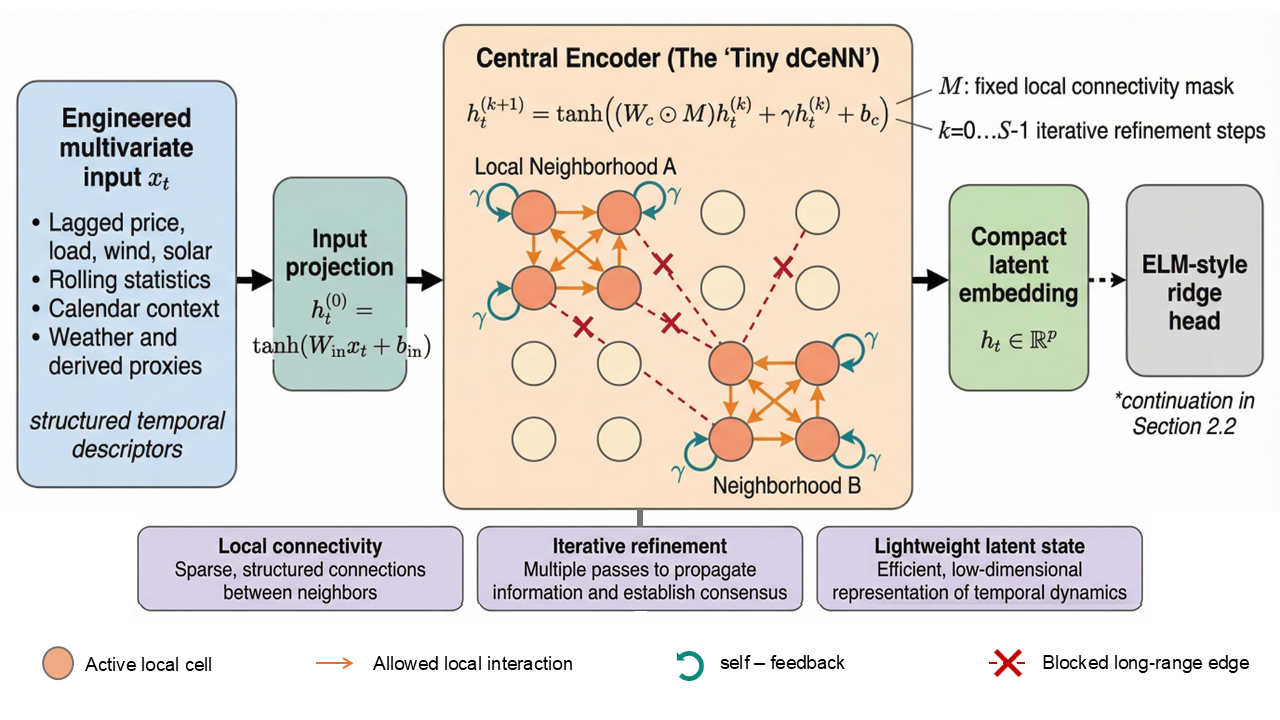
\includegraphics[width=\textwidth]{images/dCeNN_theory.png}
	\caption{Conceptual architecture of the Tiny dCeNN encoder used in the proposed framework. Engineered multivariate temporal features are first projected into an initial latent state and then refined through masked local recurrent interactions. The fixed locality mask restricts communication to neighborhood-preserving connections, while blocked long-range edges enforce structured sparsity. After iterative refinement, the encoder produces a compact latent embedding that is passed to the downstream ELM-style ridge head for forecasting.}
	\label{dCeNN_theory}
\end{figure}
\FloatBarrier   

\section{Extreme Learning Machines (ELM)}

Extreme Learning Machines were introduced as a fast-learning paradigm for single-hidden-layer feedforward networks \cite{huang2006extreme}. The central idea is that the hidden representation need not be learned by iterative backpropagation in the usual way. Instead, once the hidden-layer mapping is fixed, the output weights can be solved analytically as a linear least-squares problem. This yields very high training speed while retaining the universal approximation capability associated with sufficiently rich nonlinear hidden representations \cite{cybenko1989approximation,huang2006universal,huang2012elm_regression}.

In canonical ELM, suppose a training set contains $N$ samples $\{(\mathbf{x}_i,\mathbf{y}_i)\}_{i=1}^{N}$, where $\mathbf{x}_i \in \mathbb{R}^{d}$ and $\mathbf{y}_i \in \mathbb{R}^{m}$. For a hidden layer with $L$ nonlinear nodes, the hidden representation matrix is
\begin{equation}
H =
\begin{bmatrix}
 g(\mathbf{a}_1^{\top}\mathbf{x}_1 + b_1) & \cdots & g(\mathbf{a}_L^{\top}\mathbf{x}_1 + b_L) \\
 \vdots & \ddots & \vdots \\
 g(\mathbf{a}_1^{\top}\mathbf{x}_N + b_1) & \cdots & g(\mathbf{a}_L^{\top}\mathbf{x}_N + b_L)
\end{bmatrix},
\label{eq:elm_hidden}
\end{equation}
where $g(\cdot)$ is a nonlinear activation, and $\mathbf{a}_\ell,b_\ell$ are the hidden-node parameters. In standard ELM these hidden parameters are randomly assigned and then kept fixed. The learning problem reduces to finding the output-weight matrix $\beta \in \mathbb{R}^{L \times m}$ such that
\begin{equation}
H\beta \approx Y,
\end{equation}
where $Y \in \mathbb{R}^{N \times m}$ stacks the target vectors.

The unregularized least-squares solution is
\begin{equation}
\beta = H^{\dagger}Y,
\label{eq:elm_pinv}
\end{equation}
where $H^{\dagger}$ denotes the Moore--Penrose pseudoinverse. In practice, ridge regularization is often preferred for numerical stability and generalization \cite{hoerl1970ridge,huang2012elm_regression}. The regularized solution becomes
\begin{equation}
\beta = \left(H^{\top}H + \lambda I\right)^{-1}H^{\top}Y,
\label{eq:elm_ridge}
\end{equation}
where $\lambda > 0$ is the regularization parameter. Equation \eqref{eq:elm_ridge} is especially attractive in small and medium-sized problems because it avoids iterative gradient-based training of the output layer and gives a deterministic closed-form estimator.

The main advantage of ELM is that, once the nonlinear hidden representation is
available, the output weights can be fitted analytically rather than through
iterative backpropagation. This provides fast training while retaining the
approximation capability of a sufficiently expressive hidden representation
\cite{cybenko1989approximation,huang2006universal}.

The present thesis adopts the \emph{ELM principle} rather than a strictly classical random-hidden-layer ELM. Specifically, the hidden representation is not generated by random nodes alone; it is supplied by the dCeNN encoder described in Section 2.1. Let $\mathbf{h}_t \in \mathbb{R}^{p}$ denote the encoded latent representation of the feature vector $\mathbf{x}_t$. Stacking all encoded training samples yields a latent design matrix $H \in \mathbb{R}^{N \times p}$. The multivariate forecast targets are then obtained through
\begin{equation}
\hat{Y} = H W,
\label{eq:elm_head}
\end{equation}
where $W \in \mathbb{R}^{p \times m}$ is learned using the ridge-regularized solution in \eqref{eq:elm_ridge}. Hence, the dCeNN performs representation learning, while the ELM-style head performs analytical prediction. This hybridization is important: it retains the training-speed advantage of ELM at the output stage while allowing the latent representation to be more structured and domain-adaptive than a purely random hidden layer.

The linear output mapping also supports efficient joint prediction of correlated
targets such as solar capacity factor, wind capacity factor, load, and price.
Consequently, the ELM-style head is suitable for rapid retraining and compact
multivariate forecasting.

\FloatBarrier
\begin{figure}[H]
	\centering
	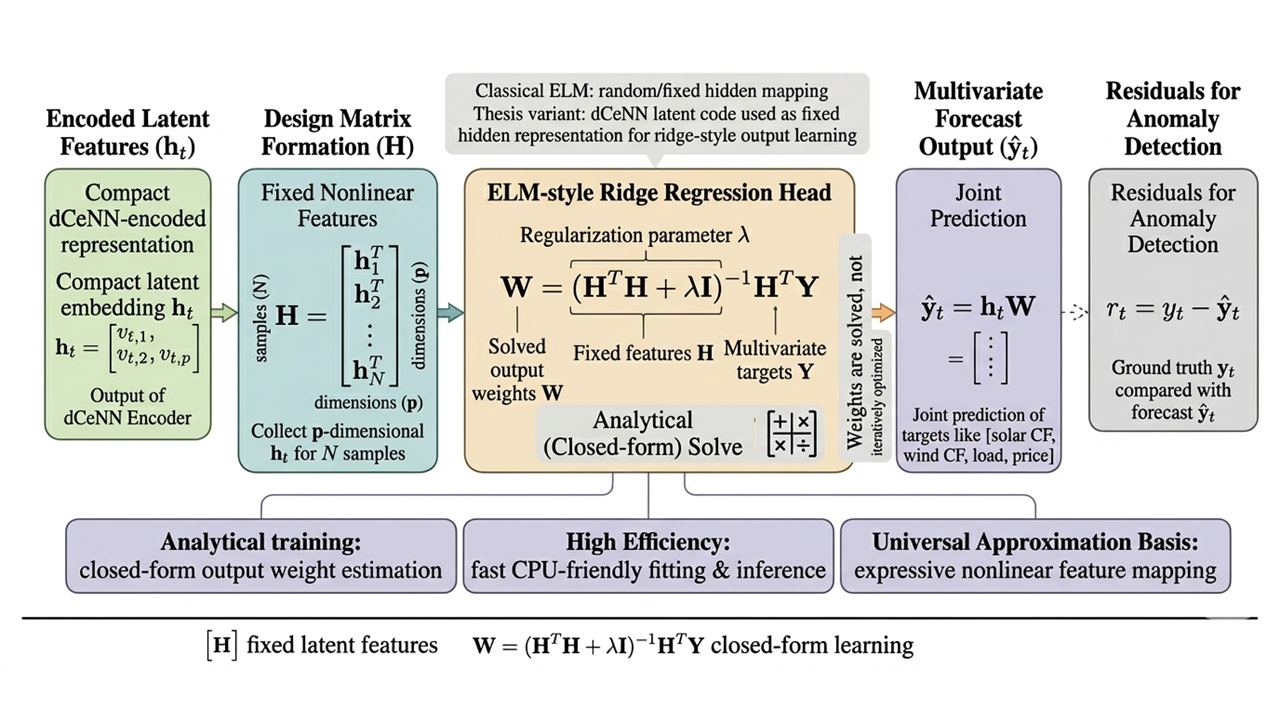
\includegraphics[width=\textwidth]{images/ELM_theory.png}
	\caption{Conceptual illustration of the ELM-style ridge regression head used in the proposed framework. The compact latent representation produced by the Tiny dCeNN encoder is treated as a fixed hidden feature matrix, while the output weights are learned analytically through a ridge-regularized closed-form solution. This enables efficient multivariate forecasting without iterative output-layer backpropagation, and the resulting predictions are subsequently used to compute residuals for anomaly detection.}
	\label{ELM_theory}
\end{figure}
\FloatBarrier

\section{Answer Set Programming (ASP)}

Answer Set Programming is a declarative problem-solving paradigm based on logic
programming and non-monotonic reasoning
\cite{gelfond1988stable,brewka2011asp,gebser2012answer}. Rather than specifying a
procedural sequence of operations, the modeler expresses the facts, rules,
defaults, exceptions, and constraints that define an acceptable solution. This
makes ASP suitable for domains in which decisions must satisfy explicit contextual
or domain-specific conditions.



The formal semantics that underpins ASP is the \emph{stable model semantics} introduced by Gelfond and Lifschitz \cite{gelfond1988stable}. Under this semantics, a logic program can have one or more \emph{stable models} (also called \emph{answer sets}), each representing a self-consistent set of conclusions supported by the rules of the program. A modern ASP solver such as \texttt{clingo} takes a collection of facts and rules, grounds the symbolic program, and computes stable models efficiently \cite{gebser2019multi}. This makes ASP particularly attractive for rule-based post-processing in machine learning pipelines.

A typical ASP rule has the form
\begin{equation}
\texttt{head} \leftarrow \texttt{body}_1,\ldots,\texttt{body}_k,\ \texttt{not}\ \texttt{body}_{k+1},\ldots,\texttt{not}\ \texttt{body}_{n},
\label{eq:asp_rule_generic}
\end{equation}
which can be read as: the \texttt{head} is true if all positive body literals hold and no negated-by-failure body literal can be established. The operator \texttt{not} expresses default negation, allowing the program to reason with incomplete information. This ability to handle defaults and exceptions is essential in domains where rules are context-sensitive rather than absolute.

In the present thesis, ASP is used as a symbolic refinement layer on top of the statistical anomaly detector. The machine-learning stage produces candidate anomalies and contextual facts; these are translated into ASP facts such as \texttt{anomaly(price,t)}, \texttt{holiday(t)}, or \texttt{pred(shortwave\_radiation,R,t)}. The rule base then decides which anomaly candidates are logically acceptable. Representative rules from the implemented framework can be summarized as follows:
\begin{lstlisting}[style=asprules,caption={Representative ASP refinement rules.},label={lst:asp_rules}]
persistent(G,T) <- anomaly(G,T), anomaly(G,T-1), anomaly(G,T-2).
invalid_solar(T) <- anomaly(cf_solar,T), pred(shortwave_radiation,R,T), R <= 0.
confirmed_economic_spike(T) <- anomaly(price,T), anomaly(load_mw,T).
valid_anomaly(G,T) <- persistent(G,T), not holiday(T), not invalid_solar(T).
valid_anomaly(price,T) <- confirmed_economic_spike(T), not holiday(T).
\end{lstlisting}
Listing~\ref{lst:asp_rules} shows representative ASP refinement rules used to validate or suppress statistical anomaly candidates.

These rules illustrate how statistical candidates are examined using explicit
domain knowledge. Candidates may be rejected because they occur under an
explainable calendar condition, conflict with radiation information, or violate a
specified physical constraint. Conversely, co-occurring signals, such as
simultaneous price and load anomalies, can provide supporting evidence for a
candidate.

This symbolic layer makes the refinement process traceable and maintainable:
decisions can be associated with explicit rules, and domain knowledge can be
updated without retraining the forecasting model. The complete rule design and
its integration with the statistical detector are presented in Chapter~4 and
Appendix~A.

\section{Conformal Prediction \& Thresholding}

After the dCeNN--ELM forecaster produces predictions, anomaly detection is based on the deviation between the observed and predicted targets. Let $y_t^{(j)}$ and $\hat{y}_t^{(j)}$ denote, respectively, the observed and predicted value of target $j$ at time $t$. The residual is
\begin{equation}
r_t^{(j)} = y_t^{(j)} - \hat{y}_t^{(j)},
\label{eq:residual_def}
\end{equation}
and the corresponding nonconformity score is taken as the absolute residual,
\begin{equation}
a_t^{(j)} = \left|r_t^{(j)}\right|.
\label{eq:nonconformity_abs}
\end{equation}
The rationale is simple: when the forecasting model has learned normal system dynamics adequately, normal observations should produce moderate residuals, whereas abnormal observations should induce unusually large residuals.

Conformal prediction provides a principled framework for transforming such residuals into uncertainty-calibrated decision rules \cite{shafer2008tutorial}. In standard split conformal prediction, a calibration set is used to compute nonconformity scores, and empirical quantiles of these scores are then used to construct prediction regions with finite-sample marginal coverage under exchangeability assumptions. For a scalar target, a conformal prediction interval can be written as
\begin{equation}
\mathcal{C}_{1-\alpha}(\mathbf{x}_t) = \left[\hat{y}_t - q_{1-\alpha},\ \hat{y}_t + q_{1-\alpha}\right],
\label{eq:conformal_interval}
\end{equation}
where $q_{1-\alpha}$ is the empirical $(1-\alpha)$-quantile of calibration residuals. An observation falls outside this interval when its residual is unusually large relative to the calibration distribution.

In this thesis, the same idea is adapted from prediction-set construction to anomaly thresholding. For each target $j$, the validation set is used as a calibration set, and the threshold is defined as an empirical quantile of absolute residuals,
\begin{equation}
\tau_j = Q_{\kappa}\!\left(\left\{ a_i^{(j)} : i \in \mathcal{V} \right\}\right),
\label{eq:global_threshold}
\end{equation}
where $\mathcal{V}$ is the validation index set and $Q_{\kappa}(\cdot)$ denotes the empirical quantile at level $\kappa$. The implemented system uses a conformal-style calibration with $\kappa = 0.90$, which yields a target-specific threshold learned directly from validation residual behavior. A statistical anomaly candidate is then declared whenever
\begin{equation}
\mathbb{I}_{\mathrm{anom}}^{(j)}(t) = \mathbb{I}\!\left(a_t^{(j)} > \tau_j\right).
\label{eq:basic_flag}
\end{equation}

Because electricity time series are strongly context-dependent, this thesis further extends the thresholding mechanism through \emph{bucketed calibration}. Let $b(t)$ denote a context bucket, such as hour-of-day or holiday status. Then the threshold becomes
\begin{equation}
\tau_j^{\bigl(b(t)\bigr)} = Q_{\kappa}\!\left(\left\{ a_i^{(j)} : i \in \mathcal{V},\ b(i)=b(t) \right\}\right).
\label{eq:bucket_threshold}
\end{equation}
Bucketed calibration accounts for variations in forecast uncertainty across
operating contexts. In the implemented framework, hour-wise thresholds are used
so that naturally volatile periods are not evaluated using the same residual
tolerance as more predictable periods.



To aggregate deviations across multiple targets, the framework defines a combined anomaly score,
\begin{equation}
S_t = \sum_{j=1}^{m} \max\!\left(0, \frac{a_t^{(j)}}{\tau_j^{\bigl(b(t)\bigr)} + \varepsilon} - 1 \right),
\label{eq:combined_score_theory}
\end{equation}
where $\varepsilon > 0$ is a small numerical constant. Equation \eqref{eq:combined_score_theory} has an intuitive interpretation: only residuals that exceed their calibrated thresholds contribute to the score, and larger exceedances contribute more strongly. This yields a severity measure that is sensitive both to the number of affected targets and to the extent of their threshold violations.

Classical conformal guarantees rely on exchangeability, whereas electricity time
series contain serial dependence, seasonality, and regime changes. The method
used here is therefore described as \emph{conformal-style residual calibration}
rather than as a strict finite-sample coverage guarantee. Its role is to derive
data-adaptive anomaly thresholds from validation residuals instead of selecting
fixed tolerances arbitrarily. The subsequent symbolic refinement of the resulting
candidates is developed in Chapter~4.

\FloatBarrier
\begin{figure}[H]
	\centering
	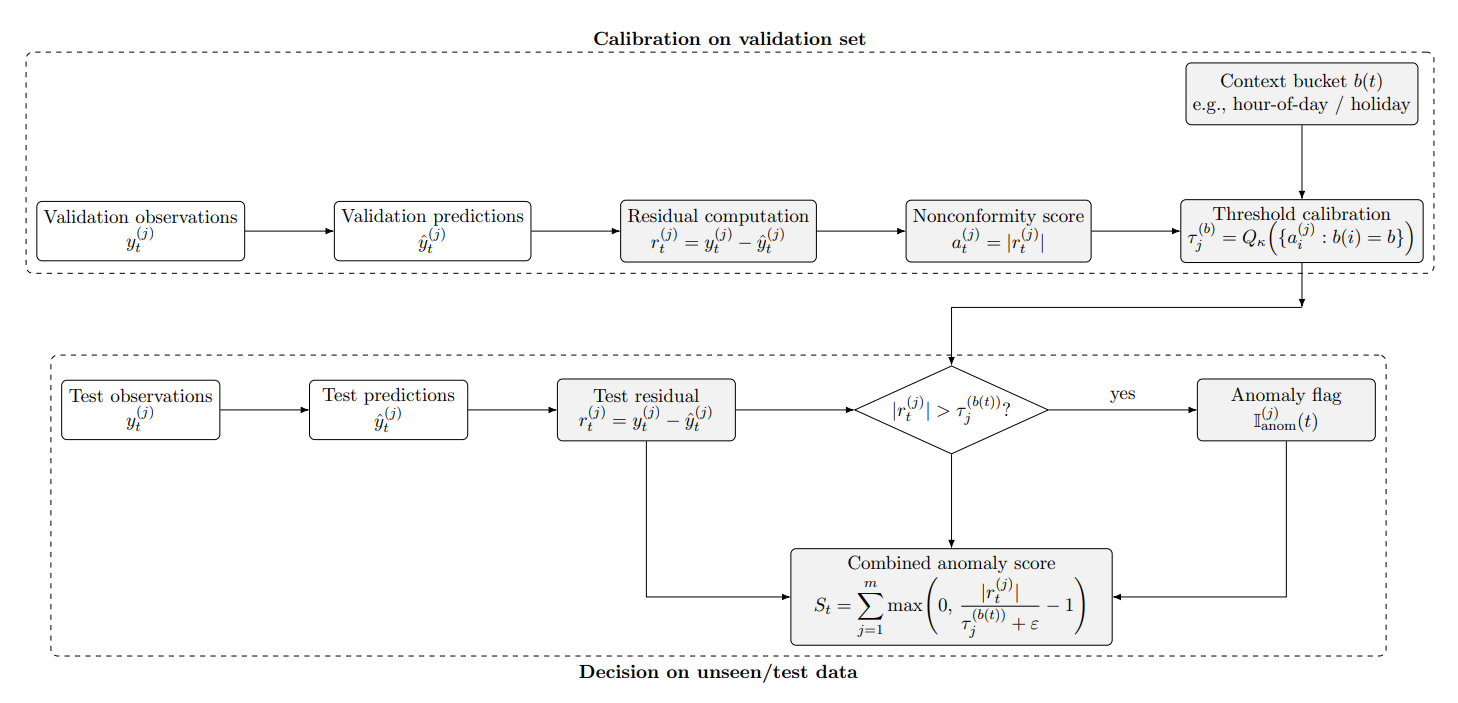
\includegraphics[width=\textwidth]{images/Threshould.png}
	\caption{Conformal-style residual thresholding pipeline. Validation residuals are converted into absolute nonconformity scores, from which target-specific thresholds are estimated as empirical quantiles, optionally within context buckets such as hour-of-day or holiday state. At test time, observed residuals are compared against these calibrated thresholds to produce anomaly flags and a combined anomaly severity score.}
	\label{Threshould}
\end{figure}
\FloatBarrier 

\FloatBarrier

\begin{table}[H]
\centering
\caption{Core theoretical components of the proposed framework.}
\label{tab:theory_components}
\begin{tabular}{|p{3.2cm}|p{4.2cm}|p{5.2cm}|}
\hline
\textbf{Component} & \textbf{Theoretical role} & \textbf{Role in this thesis} \\
\hline
Discrete Cellular Neural Network (dCeNN) & Nonlinear representation learning with local interactions and iterative state updates & Encodes engineered temporal features into a compact latent state using masked local recurrent connectivity \\
\hline
Extreme Learning Machine (ELM) & Fast analytical learning of output weights on fixed hidden representations & Maps dCeNN latent codes to multivariate forecasts through ridge-regularized closed-form regression \\
\hline
Answer Set Programming (ASP) & Declarative reasoning under stable-model semantics & Filters statistical anomalies using persistence, holiday, radiation, wind-ramp, and co-anomaly rules \\
\hline
Conformal thresholding & Calibration of uncertainty from validation residuals & Converts residuals into adaptive per-target anomaly thresholds, optionally bucketed by context \\
\hline
\end{tabular}
\end{table}

\FloatBarrier